\documentclass[11pt,oneside,letterpaper]{article}

% graphicx package, useful for including eps and pdf graphics
\usepackage{graphicx}
\DeclareGraphicsExtensions{.pdf,.png,.jpg}

% basic packages
\usepackage{color} 
\usepackage{parskip}
\usepackage{float}

% text layout
\usepackage{geometry}
\geometry{textwidth=15cm} % 15.25cm for single-space, 16.25cm for double-space
\geometry{textheight=22cm} % 22cm for single-space, 22.5cm for double-space

% helps to keep figures from being orphaned on a page by themselves
\renewcommand{\topfraction}{0.85}
\renewcommand{\textfraction}{0.1}

% bold the 'Figure #' in the caption and separate it with a period
% Captions will be left justified
\usepackage[labelfont=bf,labelsep=period,font=small]{caption}

% review layout with double-spacing
%\usepackage{setspace} 
%\doublespacing
%\captionsetup{labelfont=bf,labelsep=period,font=doublespacing}

% cite package, to clean up citations in the main text. Do not remove.
\usepackage{cite}
%\renewcommand\citeleft{(}
%\renewcommand\citeright{)}
%\renewcommand\citeform[1]{\textsl{#1}}

% Remove brackets from numbering in list of References
\renewcommand\refname{\large References}
\makeatletter
\renewcommand{\@biblabel}[1]{\quad#1.}
\makeatother

\usepackage{authblk}
\renewcommand\Authands{ \& }
\renewcommand\Authfont{\normalsize \bf}
\renewcommand\Affilfont{\small \normalfont}

% comments
\usepackage{ulem}
\definecolor{purple}{rgb}{0.459,0.109,0.538}
\def\tb#1#2{\sout{#1} \textcolor{purple}{#2}} 
\def\tbc#1{\textcolor{purple}{[#1]}}



%%% TITLE %%%
\title{\vspace{1.0cm} \LARGE \bf fluB}

\author[1]{Gytis Dudas}
\author[2]{Trevor Bedford}
\author[1]{Samantha Lycett}
\author[1,3]{Andrew Rambaut}

\affil[1]{Institute of Evolutionary Biology, University of Edinburgh, Edinburgh, UK}
\affil[2]{Vaccine and Infectious Disease Division, Fred Hutchinson Cancer Research Center, Seattle, WA, USA.}
\affil[3]{Fogarty International Center, National Institutes of Health, Bethesda, MD, USA.}

\date{\today}

\begin{document}
\maketitle

\begin{abstract}

Influenza B viruses are increasingly being recognized as major contributors to morbidity attributed to seasonal influenza. 
Currently circulating influenza B isolates are known to belong to two antigenically distinct lineages referred to as B/Victoria and B/Yamagata lineages on the basis of haemagglutinin inhibition (HI) assays. 
Frequent reassortment between the segments of these two lineages has been noted in the past \cite{lindstrom1999}, but the effects of these reassortments have not been investigated in much detail.

\end{abstract}

\pagebreak


\section*{Introduction}
Seasonal influenza causes an estimated 250,000 to 500,000 deaths annually and is comprised of three virus types (influenza A, B and C) co-circulating in humans, of which influenza A is considered to cause the majority of seasonal morbidity and mortality.
Though lacking the degree of antigenic diversity that influenza A viruses possess, influenza B viruses are increasingly being recognized as important human pathogens \cite{paul-glezen2013}.
Following the 2009 A/H1N1 pandemic, influenza B has increased in prevalence and in the 2012/2013 European season as many as 53\% of influenza sentinel surveillance samples tested positive for influenza B \cite{ECDC1213}. 

Like all members of \textit{Orthomyxoviridae}, influenza B viruses have segmented genomes, which allow viruses co-infecting the same cell to exchange segments (a process known as reassortment). 
Influenza A viruses are widely considered to be a major threat to human health worldwide due to the ability to cause pandemics in humans via reassortment of seasonal human and non-human influenza A strains. 
The only known persistent source of influenza B viruses are humans (and occasionaly seals \cite{osterhaus2000,bodewes2013}), thus limiting the virus's available antigenic reservoir. 
It has been suggested that influenza B viruses use a combination of reassortment and point mutations to generate antigenic diversity \cite{nerome1998,mccullers1999}.

Currently circulating influenza B viruses are comprised of two antigenically distinct lineages -- Victoria and Yamagata (referred to as Vic and Yam, respectively) -- named after two strains, B/Victoria/02/87 and B/Yamagata/16/88, which possess antigenically distinct haemagglutinin (HA) surface glycoproteins. 
The two HA lineages still co-circulate today and are thought to have shared a most recent common ancestor in xxxx. 
All other influenza B segments also show a split in xxxx (comment - our estimate \textit{circa} 1984 figure \ref{TMRCAhpd}, use a figure to show TMRCAs and rates for each segment?), although the numbers of strains falling on either side of the split are different due to reassortments following the initial split of Yam and Vict lineages in all segments and fixation of one or the other lineage in some segments.

%\begin{figure}[h]
%	\centering		
%	\includegraphics[width=0.95\textwidth]{figures/InfBtmrcaHPD}
%	\caption{\textbf{Provisional TMRCA plot.}}
%	\label{TMRCAhpd}
%\end{figure}

Previously, through the use of time-stamped phylogenetic trees, the reassortment history of major clades of influenza B has been reconstructed \cite{chen2008}, showing extensive and often complicated patterns of reassortment between all segments of influenza B viruses both between and within Vic and Yam lineages.
Another approach exists, however, whereby belonging to either the Victoria or Yamagata lineage in the tree of one segment can be used as a discrete trait in trees of other segments.
Reassortment events which result in the replacement of one segment lineage by another show up as changes in the discrete trait along a branch and allow the inference of parameters related to the subtree descended from the node displaying a changed trait (see Figure \ref{methodFig}).
Here, we use discrete traits to model inter-lineage reassortments between Victoria and Yamagata lineage segments in BEAST to look at lineage persistence times following reassortment events. 
We show that despite extensive reassortment, PB1, PB2 and HA segments of influenza B viruses still survive as Victoria and Yamagata lineages, which appear to be co-adapted to the point where virions which do not contain PB1, PB2 or HA segments derived entirely from either the Vic or the Yam lineage are selected against and, to the best of our knowledge, have not been sampled since 1996.
In other segments (PA, NP, NA, MP and NS) a single lineage has been fixed in the influenza B population: Yam for PA, NP, NA and MP and Vic for NS.

\begin{figure}[h]
 \centering		
	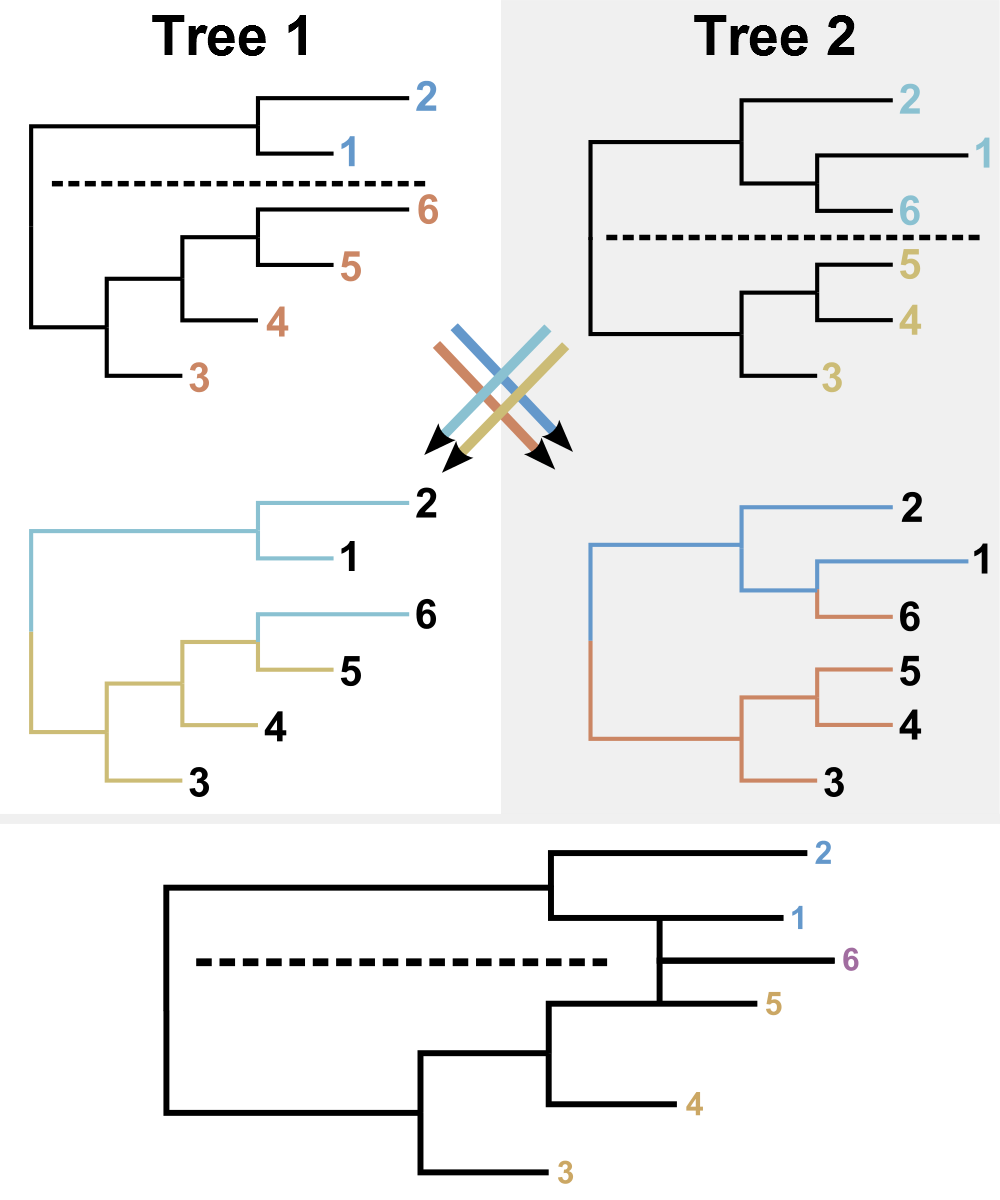
\includegraphics[width=0.45\textwidth]{figures/TreeFigure2}
	\caption{\textbf{Schematic depiction of method.}}
	\label{methodFig}
\end{figure}

\section*{Methods}

\subsection*{Sequences and subtyping}
We compiled a dataset of 452 complete influenza B genomes from GISAID (comment - need acknowledgment tables). 
Each strain was assigned to a lineage (either Vic or Yam) in each segment by making maximum likelihood trees and looking whether it fell within the subtree containing B/Victoria/02/87 or B/Yamagata/16/88 sequences with the exception of the NS segment (B/Victoria/02/87 was a reassortant and possessed a Yam lineage NS), where B/Norway/1/84 (comment - B/Czechoslovakia/69/1990 could be used as well, since it is the only strain showing an entirely Vic genome) was considered as being representative of Victoria lineage.
Each strain was thus assigned 8 lineages depending on the combination of lineages it belongs to in all trees (for example all segments except for NS in strain B/Victoria/02/87 belong to Vic lineage and can thus be represented as V,V,V,V,V,V,V,Y). 
Seven of these where then used as discrete states in each of the trees (e.g. PB1 tree had PB2, PA, HA, NP, NA, MP and NS as traits and V or Y as trait values) in BEAST (comment - reference BEAST).

\subsection*{Building trees}
Temporal phylogenies were recovered for each segment using the HKY model of nucleotide substitution, 3 codon partitions, robust counting (comment - reference robust counting) and GMRF Bayesian skyride (comment - reference skyride) as the demographic model over the course of an MCMC chain (3 parallel runs of 200 million states, sampling every 20000 steps).
In addition we used `relaxed' tips for 94 sequences (of which 93 only had year of isolation and 1 had only year and month of isolation) \tbc{CITE}.
We inferred the ancestral state of lineages in each segment by using discrete traits (asymmetric CTMC matrix with BSSVS (comment - cite Philippe)). Because the posterior set of trees have branches labelled with the inferred lineage in all other segments, we can detect inter-lineage reassortments whenever a trait transition is observed (i.e. Y to V or V to Y) between a node and its descendant in any segment. 
In addition, by reconstructing the ancestral state of all other genomic segments jointly we can infer co-reassortment events when more than one trait transition occurs on the same node in a tree.

We use a measure of persistence which is defined as the ratio of distances (in units of time) between a reassortant node and its most recent tip (the event is sampled uniformly over the branch displaying a trait value that is different from its parent node) and compare it to the mean of distances between all nodes and their respective most recent tips. 
If this statistic is below 1 a reassortment event is presumed to be disadvantageous, if it is above 1 the event is presumed to be advantageous.

Alternative:
We start by allocating the tips in the tree to yearly bins starting from 1984 and ending in 2013. 
At each state of the MCMC chain we choose a random tip from each bin and traverse the tree towards the root until a reassortment event (i.e. a trait switch) is encountered.
We log the traits which have transitioned at the reassortant node (i.e. the reassorting segment), the direction of transition (e.g. whether the parental node was V and the child node Y or vice versa) and the amount of time separating the tip and the node displaying a trait transition. 
The time taken to traverse back to a reassortment event is expected to be longer for advantageous reassortments than for non-advantageous reassortments.

\subsection*{Building a consensus set of reassortment events}
Maximum clade credibility trees were made after discarding the first 1000 trees as burnin. 
Nodes with trait values different from the trait value of their parental node were classified as being reassortants.
The persistence time, descendant tips and reassorting segments were logged for each reassortant node and aggregated across analyses based on descendant tips.

\subsection*{Measures of diversity}
We inferred the diversity of each segment over time by finding the oldest most recent common ancestor of all branches existing at yearly intervals, which places an upper boundary on diversity existing at each time period.
In addition, we calculated mean pairwise TMRCA between branches inferred to be in virions possessing Vic and Yam lineage PB1, PB2 and HA.


\subsection*{Work in progress}
Currently running "null" traited trees where trait maps have been rearranged (keeping the same ratio of trait values).


\section*{Results}

\subsection*{PA, NP, NA, MP and NS segments have periodically lost diversity}
The split of Vic and Yam lineages can be found in all segments.
Following the split of the two lineages, each segment could be assigned to either Vic or Yam lineage and inter-lineage reassortment events have yielded mixed-lineage genome constellations.
Some viruses with mixed-lineage genomes have become common ancestors to many later strains (i.e. the "trunk" of the phylogenetic tree) and the segment lineages involved so successful, as to become fixed within the influenza B population circulating today.
We find that Vic lineage PA, NP, NA and MP segments have gone extinct (i.e. no sequences from those lineages have been sampled in recent years see Figure \ref{lineageRatiosOverTime}), replaced entirely by the respective segments of Yam lineage in viruses bearing a Vic lineage HA.
Similarly, Vic lineage NS has become fixed in the viral population as well.
By looking at the oldest most recent common ancestor of all lineages existing within the tree of each segment at yearly timeslices (see Figure \ref{tmrcaOT}), it is clear that PA, NP, NA, MP and NS segments have undergone periodic losses of diversity, whereby sampled sequences trace their ancestry to increasingly more recent common ancestors.


\subsection*{PB1, PB2 and HA segments continue to circulate as two lineages and have not reassorted recently}
Unlike PA, NP, NA, MP and NS segments, which have periodically lost diversity, we find that PB1, PB2 and HA segments have continued to accumulate diversity since the initial split of Vic and Yam lineages (see Figure \ref{tmrcaOT}).
In addition, there is evidence to suggest that the numbers of sequences that belong to either Vic and Yam lineages of PB1, PB2 and HA segments have been sampled at a ratio close to 0.5 (see Figure \ref{lineageRatiosOverTime}), presumably due to the action of some form of balancing selection, possibly to maintain antigenic diversity.
Our findings suggest that the diversity in PB1, PB2 and HA segments is not maintained independently, but is very likely a result of co-adaptation between these segments.
By measuring the mean pairwise diversity between branches in each tree that were assigned either a Vic or Yam label in other segments, we look for reductions in diversity, which indicate that an inter-lineage reassortment event has taken place.
In example \ref{ARGexample}, if, over time slices, we measured mean pairwise distance between red and blue branches in tree 1, after they have been reciprocally labelled with each tip's position (with respect to some pre-defined bifurcation) in tree 2, we would find a drop in this measure, since the distance between tip 6 and tip 5 is now shorter and does not go through the root of the tree.
Thus, by measuring pairwise distances between differently labelled branches we get a sense of how panmictic different segments are with respect to each other.
If we repeat this procedure for all trees and focus on PB1, PB2 and HA lineage labels, we find that mean pairwise diversity between branches labelled as having for example, a PB1 segment of Vic or Yam lineage in PB2 and HA trees (and other combinations of the 3 trees and their labels), show small drops in diversity initially, but from the 1997 time slice onwards all branches labelled as Vic or Yam have a common ancestor at the root of the tree.
We also find evidence of co-reassortment in PB1, PB2 and HA segments: in Figure \ref{betweenDiversity} all three graphs become identical after 1997, indicating that the same PB1, PB2 and HA labels have been assigned to the same branches in trees of all other segments.
Our findings therefore suggest that a single configuration of Yam and Vic lineages of PB1, PB2 and HA segments has been preserved since the split of Vic and Yam lineages and have not reassorted with respect to each other, but rather have co-reassorted as a single unit, from 1997 onwards.

\subsection*{Victoria and Yamagata lineages of PB1-PB2-HA are co-adapted segment complexes}
We find that PB1, PB2 and HA segments, in addition to not reassorting across the Vic-Yam lineage boundary, form co-reassorting segment complexes derived entirely of Vic or Yam lineage segments.
Figure \ref{stateTime} shows the sum of branch lengths which were labelled as having entirely Vic or entirely Yam PB1, PB2 and HA segments (i.e. where a branch was labelled as having Vic PB1, Vic PB2 and Vic HA) compared to the sum of branch lengths where one or more of the labels is of another lineage (e.g. Vic PB1, Yam PB2 and Yam HA).
Together with Figure \ref{betweenDiversity} it suggests that some inter-lineage reassortment has occured between PB1, PB2 and HA segments soon after the split of Vic and Yam lineages, but the resulting viruses were not fit and did not become the trunk of the tree.
Viruses bearing mixed-lineage PB1-PB2-HA complexes had the following constellations of PB1, PB2 and HA: VVY (B/Bankok/163/1990-like), YVV (B/Nanchang/630/1994-like) and YVY (B/New York/24/1993-like).
We do not show results for other lineage labels as none of them show this pattern of reciprocally preserved diversity with any other segment.

\subsection*{Other segments evolve with considerable independence}
The reconstructed evolution of Victoria and Yamagata lineages of all segments reveals a considerable degree of autonomy.
For example, of all the Yamagata lineage segments that were reassorted into Victoria lineage PB1-PB2-HA background giving rise to B/Hong Kong/330/2001-like viruses, most segments went extinct following later reassortments, save for NP, which continued circulating until, at least, 2011.
A more dramatic example can be found in the NS segment, where the Vic lineage had been fixed in the population after reassorting into an otherwise entirely Yam-derived genome constellation and then reassorted back into a Vic lineage PB1-PB2-HA background, replacing the NS lineage that was present there. 

\begin{figure}[h]
	\centering		
	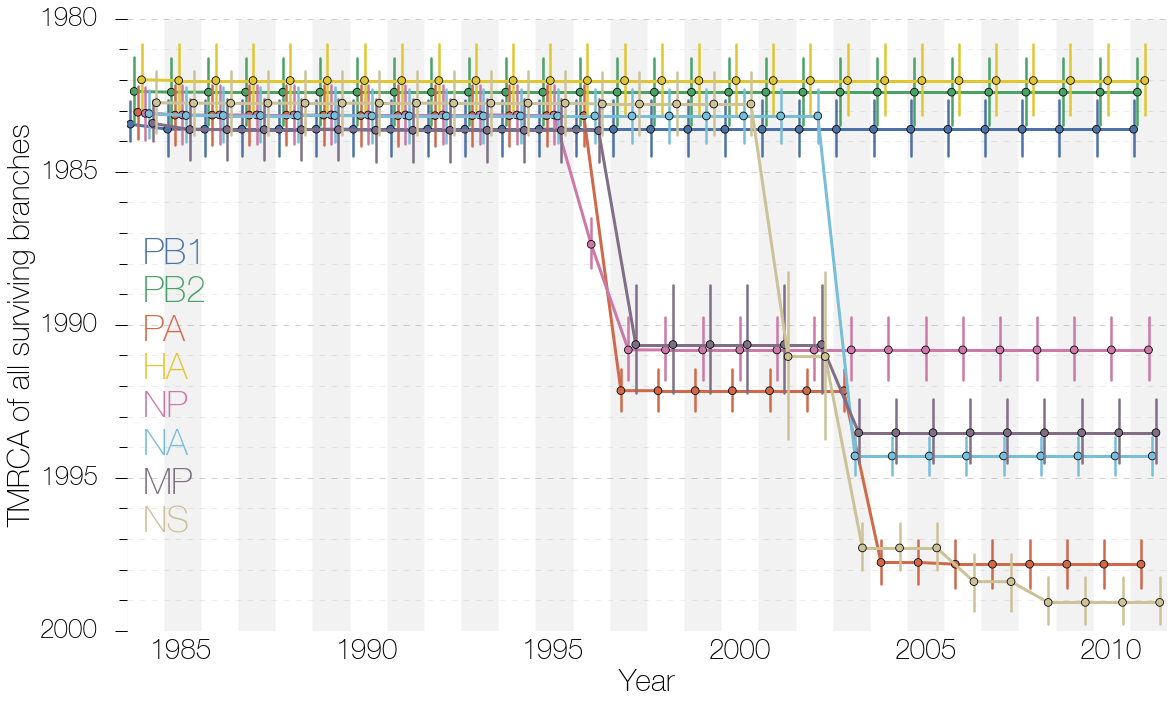
\includegraphics[width=0.95\textwidth]{figures/InfB_tmrcaOT_lines.png}
	\caption{\textbf{TMRCA over time plot.}}
	\label{tmrcaOT}
\end{figure}

(comment - need higher resolution for lineage ratios figure or switch to vector graphics)
\begin{figure}[h]
	\centering		
	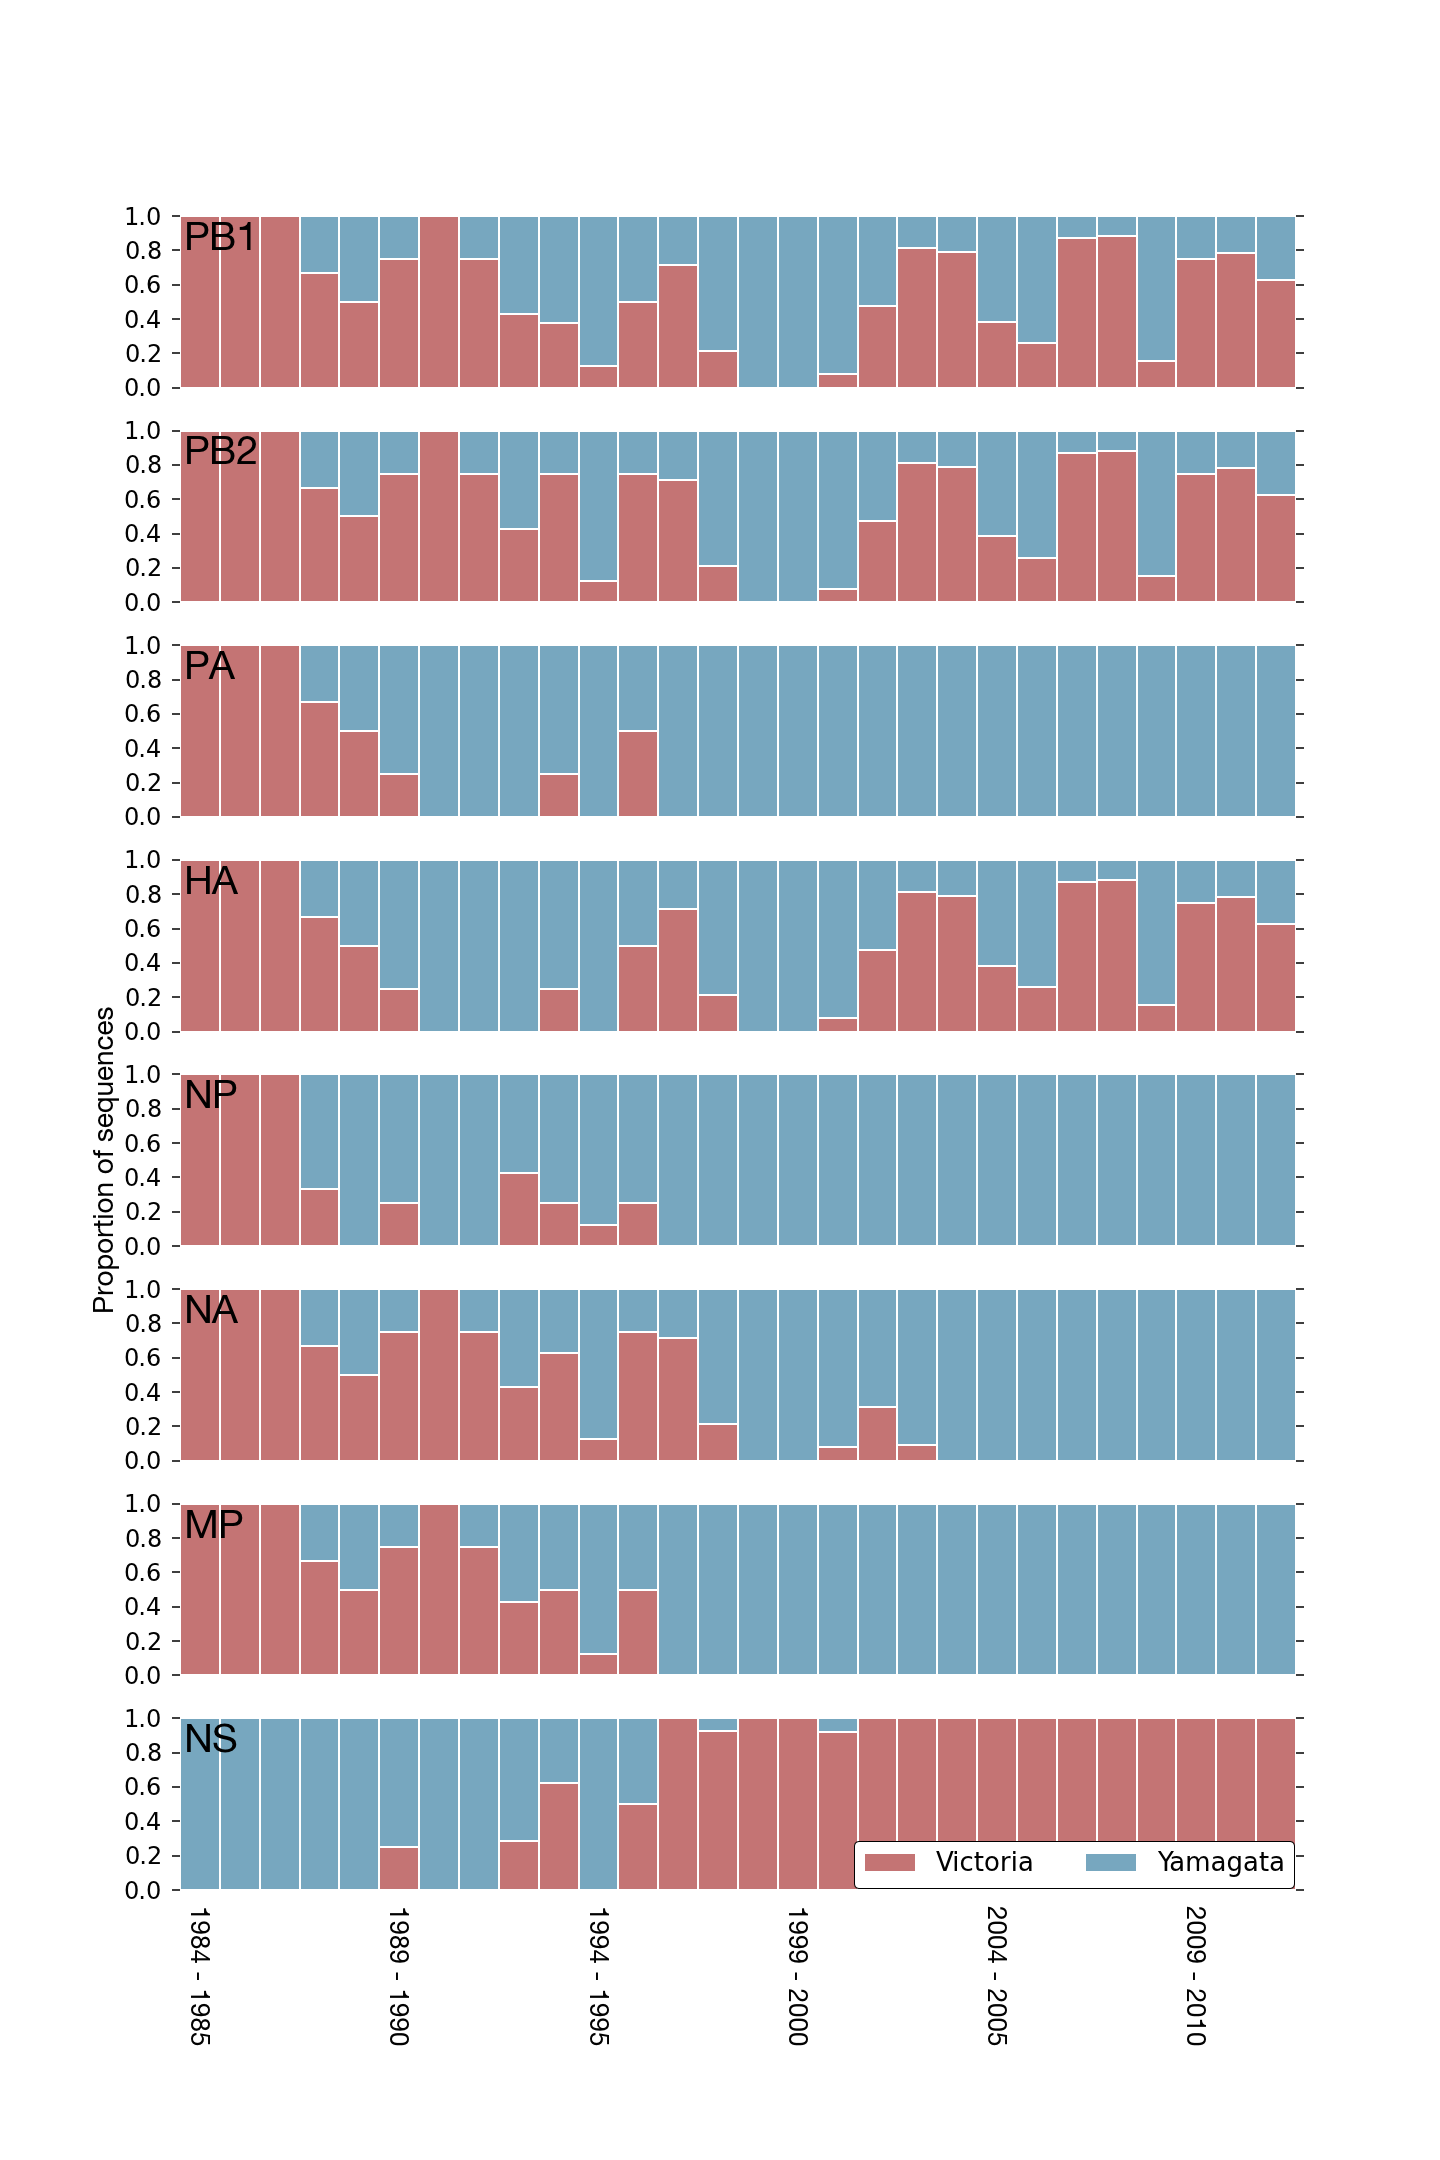
\includegraphics[width=0.55\textwidth]{figures/InfB_LineageRatiosOverTime.png}
	\caption{\textbf{Ratio of lineages in the dataset.}}
	\label{lineageRatios}
\end{figure}

\begin{figure}[h]
	\centering		
	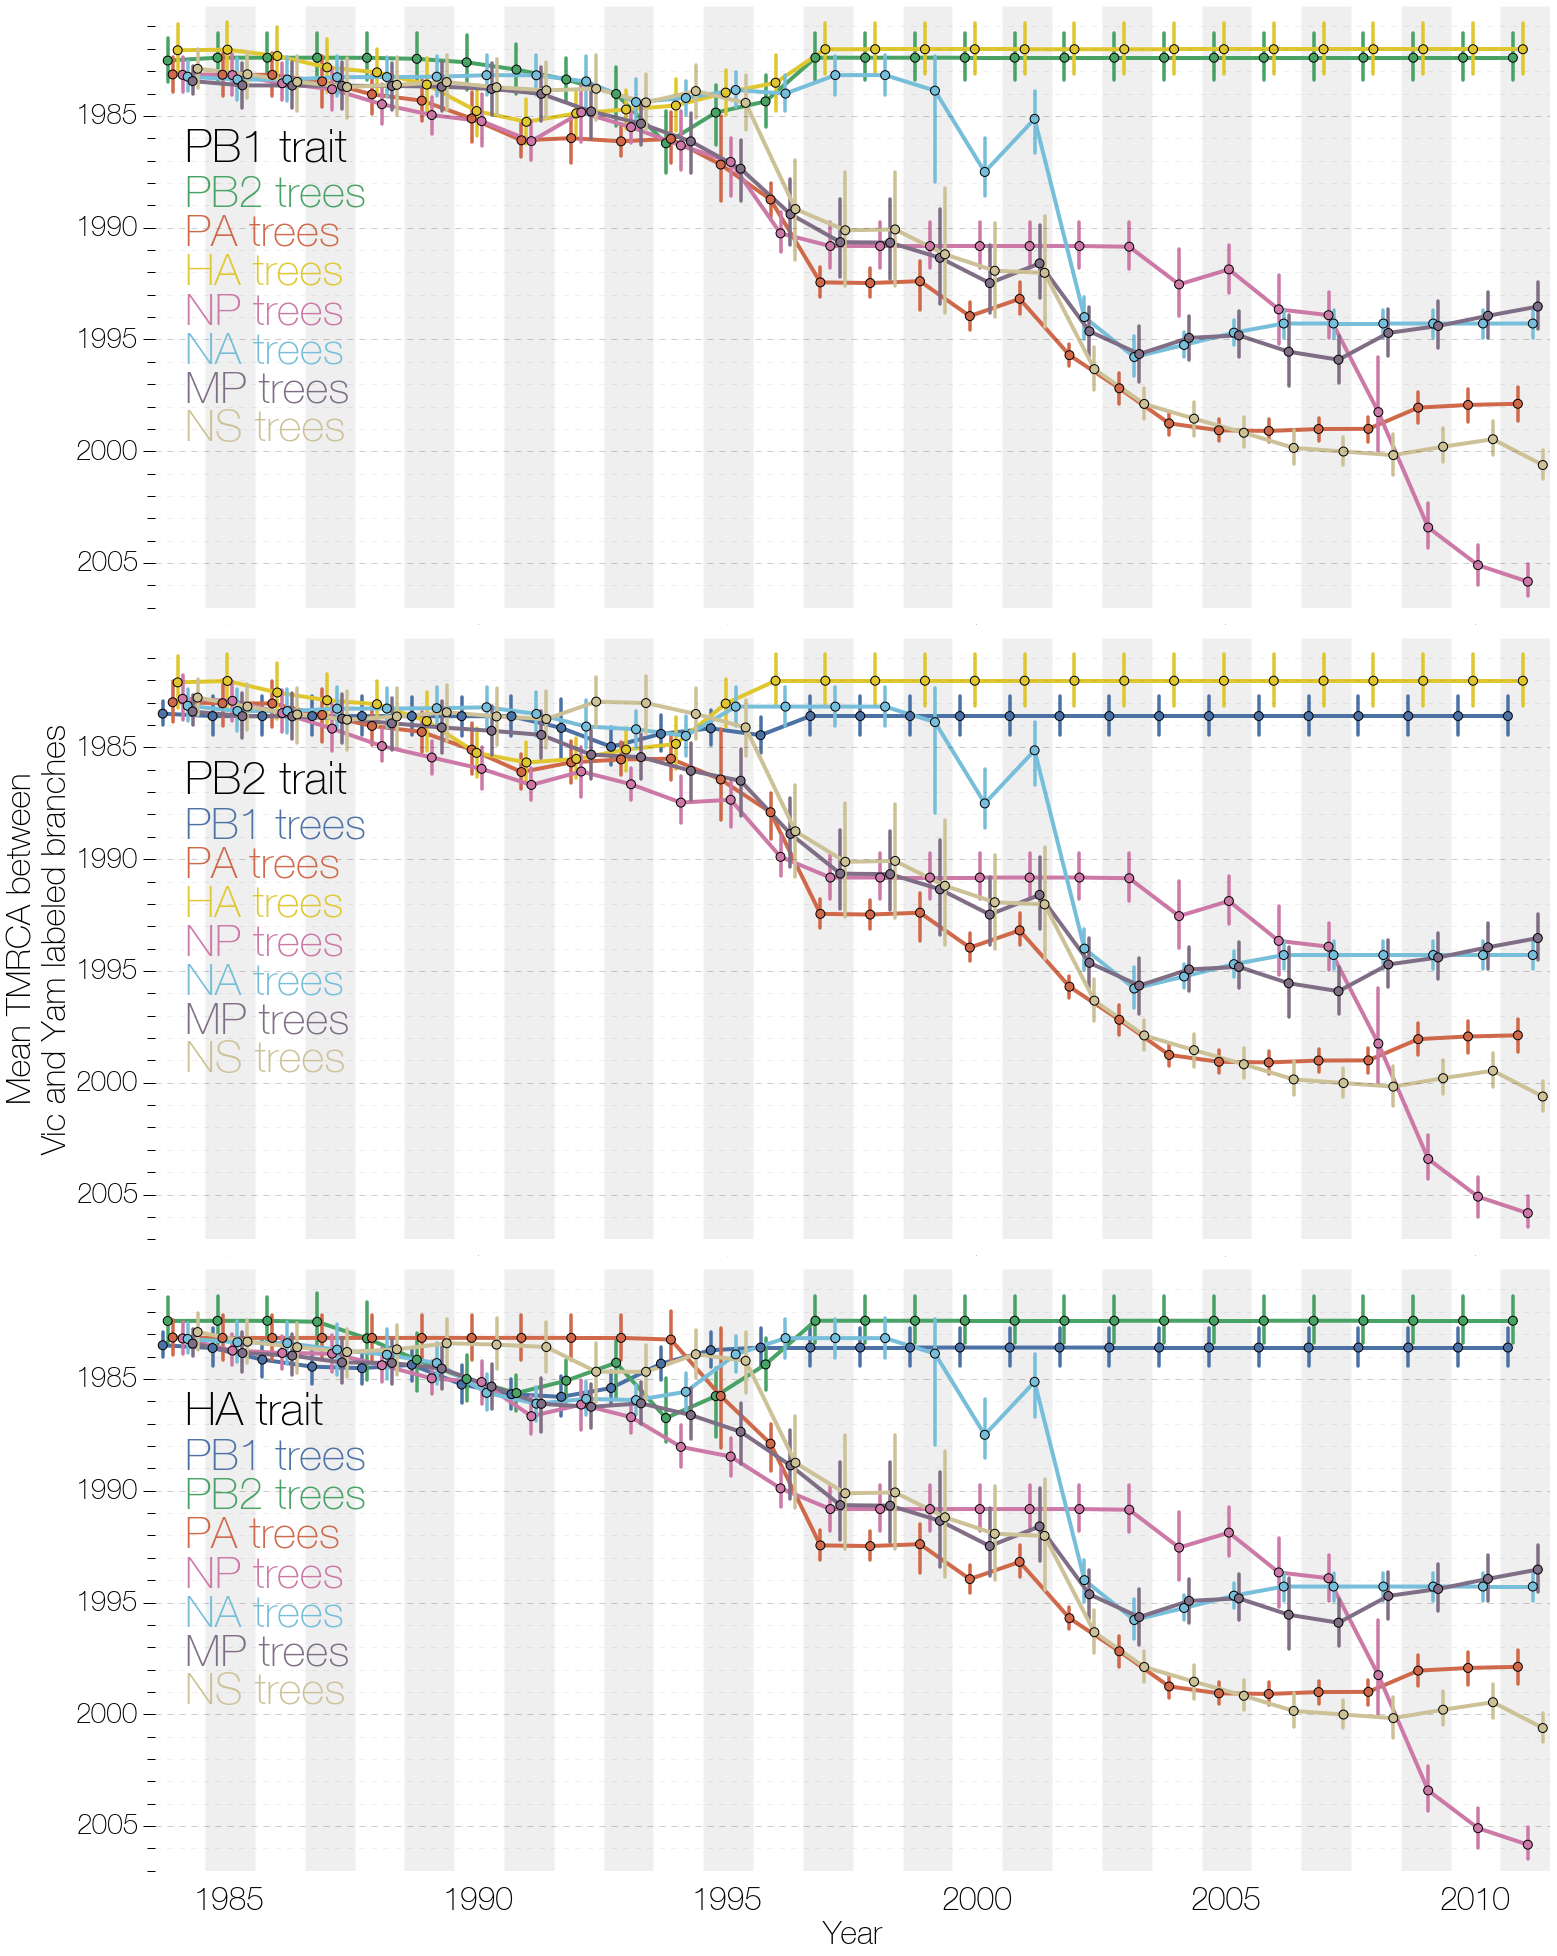
\includegraphics[width=0.95\textwidth]{figures/InfB_betweenDiversity.png}
	\caption{\textbf{Ratio of lineages in the dataset.}}
	\label{betweenDiversity}
\end{figure}

\begin{figure}[h]
	\centering		
	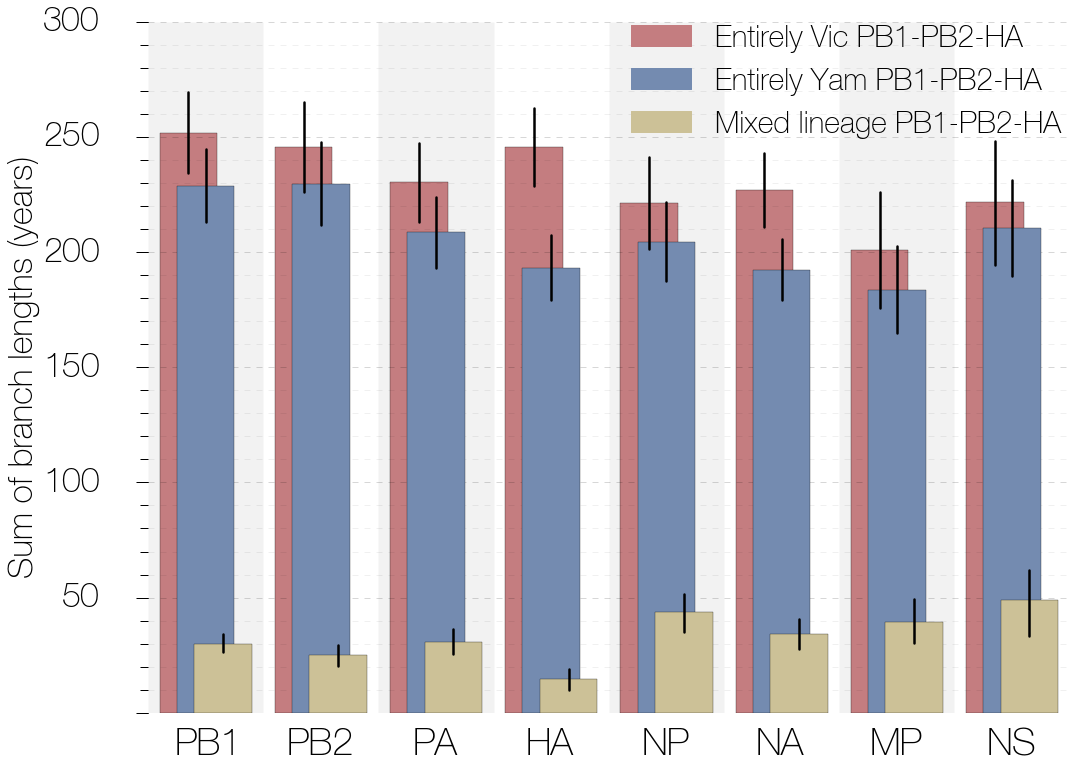
\includegraphics[width=0.95\textwidth]{figures/InfB_stateTime.png}
	\caption{\textbf{Total time spent in "pure" vs "mixed" PB1-PB2-HA}}
	\label{stateTime}
\end{figure}

\section*{Discussion}

\subsection*{Limitations of current study}
The methods used in this paper have limited power to detect reassortments, since lineages have been fixed over time and thus all viruses eventually come to bear either Vic or Yam lineage PA, NP, NA, MP and NS segments.
We can also only detect reassortment events where a lineage has switched from Vic to Yam or \textit{vice versa}, but not when a lineage has switched from a Yam lineage to another Yam lineage, which has occurred in the past (e.g. the 2004 Vic lineage PB1-PB2-HA complex reassortment with NP is only visible in the NP tree, since all viruses in our dataset from 1995 onwards, including Vic PB1-PB2-HA complex-bearing ones, had a Yamagata lineage-derived NP).

\subsection*{PB1-PB2-HA co-adaptation has evolved over time}
Our findings suggest that PB1, PB2 and HA segments of Vic and Yam lineages represent co-adapted co-reassorting segment complexes.
We argue that PB1-PB2-HA complexes have become co-dependent on each other to the extent that any reassortant viruses possessing mixed-lineage PB1-PB2-HA are unfit and possibly never get sampled or, if sampled, never persist for long enough to be fixed in the influenza B population.
Supporting this, we detect at least 3 genome constellations having mixed-lineage PB1-PB2-HA sampled early in the first decade of the split between Vic and Yam lineages, when, presumably, Vic and Yam lineages of PB1, PB2 and HA segments were still similar at the protein sequence level to produce viable, though unfit, influenza B viruses.
We interpret lack of reassortment within the PB1-PB2-HA complex across the lineage boundary in recent times as evidence of a considerable degree of co-dependence within the Vic and Yam PB1-PB2-HA lineages, whereby mixed-lineage reassortants are inviable or unsampled by surveillance due to being outcompeted by viruses with pure-lineage PB1-PB2-HA complexes.

\subsection*{Potential causes of co-dependence between PB1-PB2-HA}
Previous studies have investigated possible co-dependence patterns between segments of influenza B viruses, by focusing on segments which would be expected to be co-adapted, e.g. PB1-PB2-PA and HA-NA.
Though it would be easy to explain co-adaptation between the aforementioned segments by referring to their functional roles (e.g. PB1-PB2-PA form the polymerase heterotrimer and HA-NA have antagonistic activities), our findings suggest a more subtle relationship between PB1, PB2 and HA segments.
It is clear that PB1-PB2-HA segments do not preferentially reassort together, because there have been at least 3 sampled mixed-lineage PB1-PB2-HA complex constellations, which did not become fixed in the population and recent evidence suggests, that, at least in influenza A, reassortment between segments differing by a single synonymous difference is highly efficient \cite{marshall2013}.
In the absence of clear functional explanations of why PB1, PB2 and HA should be co-adapted, we draw attention to a recent influenza A study, which found that during the process of vaccine creation, whereby recent human influenza A isolates are reassorted with an egg-adapted strain in an attempt to reassort HA-NA of the recent isolate into the otherwise entirely egg-adapted genome background.
Cobbin et al. \cite{cobbin2013} found that the reassortant viruses following this procedure, together with the HA-NA segments the PB1 segment gets co-reassorted more frequently than expected by chance.
Cobbin et al. suggest a gene regulatory role for the PB1 segment, as its presence or absence has dramatic effects on HA concentration on the surface of virions and total virion production.
Without more, and more recent, reassortment events we cannot offer more than speculation to the nature of the relationship between PB1, PB2 and HA segments of Vic and Yam lineages.
We do however see several potential causes for the phenomenon we observe.
It would be possible that balancing selection is preserving the diversity in one segment, the others hitchhiking along.
A good candidate for this would be HA, as it is now the sole bearer of antigenic diversity within the influenza B population (NA of Vic lineage having gone extinct), until the Yam lineage NA segment under Vic PB1-PB2-HA recovers sufficient diversity.
Alternatively, either differences in gene expression or fidelity between Vic and Yam PB1 or PB2 could cause an apparent co-adaptation between PB1, PB2 and HA segments.
Finally, it is also possible that Vic and Yam lineages of PB1, PB2 and HA segments have simply become co-adapted to each other, without any one segment being the driver of diversity preservation.

\subsection*{The future of influenza B viruses}
The co-adaptation between Vic PB1-PB2-HA and Yam PB1-PB2-HA complexes is a potential insight into things to come.
We see two potential alternative paths of evolution.
One, where more segments will be recruited into these complexes, as part of a speciation process, until all circulating influenza B viruses possess genomes with segments firmly associated with either the Vic or Yam lineage PB1-PB2-HA complex.
For some time it seemed like the NP segment would be recruited into the PB1-PB2-HA complex, but recent reassortment events suggest that all Yam NP lineages reassorted into Vic lineage PB1-PB2-HA background are being outcompeted by a Yam NP lineage reassorted most recently (represented by viruses with the B/Brisbane/33/2008-like genome constellations).
Another alternative is continued reassortment of all non-PB1-PB2-HA segments between Vic and Yam PB1-PB2-HA complexes.
Finally, it is not impossible that one PB1-PB2-HA complex lineage will go extinct in the future, by chance or by being outcompeted by the other lineage, thus leaving a single-lineage influenza B population.
Given the relatively recent explosion of sequence data available for influenza B, it is difficult to say whether such two-lineage dynamics have not occurred in the distant past.
In the former two scenarios (speciation and co-circulation) we have expectations about the long term trend of reassortment.
If the influenza B population is on its way to speciation we expect that over time inter-lineage reassortment frequency should decrease, as more and more segment lineages get recruited into co-adapted segment complexes.
On the other hand, if influenza B viruses continue co-circulating as two PB1-PB2-HA lineages exchanging non-PB1-PB2-HA segments, reassortment frequency is expected to be constant.
Seeing how rarely influenza B viruses reassort across the Vic-Yam lineage boundary, the timescale for finding out which of the aforementioned scenarios, if any, are under way, is impractical at best.

\subsection*{Implications for influenza B virus control and prevention}
It is our hope that understanding the mechanism(s) underlying the links between Vic and Yam lineage PB1-PB2-HA complexes might suggest a more varied approach to both influenza B surveillance and control.
For one, our findings suggest that viruses bearing mixed-lineage PB1-PB2-HA complexes, if unveiled by surveillance, are unlikely to contribute to future influenza B evolution.
Similarly, in the absence of sequence data, it should be possible to predict the lineage of PB1, PB2 and HA segments of influenza B viruses by sequencing only one of those segments.
It remains to be seen whether equivalent or similar links exist between segments of influenza A viruses, which, by far, present a much greater threat to human health worldwide than influenza B viruses.
In addition, by discovering the underlying mechanism by which PB1, PB2 and HA are co-adapted might reveal potential cracks in the armour of influenza viruses, allowing for the creation of anti-virals to be used with currently deployed oseltamivir and zanamivir in a multi-drug approach similar to the one used against bacteria.

\subsection*{Predictions}
We see two potential future directions of research.
Using previously developed plasmid systems it would be possible to create artificial reassortants, combining Vic and Yam lineages of PB1, PB2 and HA segments.
We make two predictions for such experiments.
One, viruses with mixed-lineage PB1-PB2-HA complexes will have reduced fitness compared to pure-lineage PB1-PB2-HA complexes.
Two, if the relationship between Vic and Yam lineage PB1, PB2 and HA segments has indeed evolved over time, viruses with mixed-lineage PB1-PB2-HA complexes isolated earlier will perform better than viruses with PB1-PB2-HA isolated more recently.
However, there is potential for pleiotropic effects of other segments to interfere with fitness measurements.
A second approach is to use sequence data to look for linkage disequilibrium between polymorphisms on PB1, PB2 and HA segments of Vic and Yam lineages.
Polymorphisms originating close in time on different segments of Vic and Yam lineages could be used to infer the sites potentially responsible for the observed co-adaptation of PB1, PB2 and HA segments.
This could then pave way for wet-lab experiments where, for example, Vic PB1, PB2 or HA segments would be manipulated at potential sites to get Yam-like segments, which after being reassorted into Yam genome constellations should give reassortants of similar fitness to viruses with entirely Yam-derived PB1-PB2-HA complexes. 

\section*{Conclusions}
In this study we have investigated the patterns of reassortment amongst two influenza B virus segment lineages and found consistent co-reassortment of 3 segments: PB1, PB2 and HA.
Our findings reveal that Vic and Yam PB1, PB2 and HA segments co-associate amongst themselves with segments of their own lineage, thus resulting in an entirely Vic-lineage-derived PB1-PB2-HA segment complex and an entirely Yam-lineage-derived PB1-PB2-HA segment complex.
Though we detect strains with mixed-lineage PB1-PB2-HA complexes early after the split between Vic and Yam lineages, we find that they have performed poorly and have comprised only about 10\% of the total evolution undergone by influenza B viruses sampled in this study.
We argue that this is evidence of a selectively maintained relationship between PB1-PB2-HA complex of Vic and Yam lineages and not due to biased reassortment.
In addition, the close timing of these mixed-lineage PB1-PB2-HA reassortants close to the split of Vic and Yam lineages suggests that the relationship between each lineage's PB1-PB2-HA complexes have developed over time and in their current state are undetected by surveillance due to either poor fitness or inviability of reassortants with mixed-lineage PB1-PB2-HA complexes.



%\begin{figure}[h]
%	\centering		
%	\includegraphics[width=0.95\textwidth]{figures/InfB_TMRCAOverTime}
%	\caption{\textbf{Provisional TMRCA over time plot.}}
%\end{figure}


\bibliographystyle{pnas}
\bibliography{fluB}
\end{document}
